\documentclass[a4paper,11pt,fleqn]{jarticle}
\usepackage[dvipdfmx]{graphicx}
\usepackage{float}
\usepackage{amsmath}
\usepackage{fancyhdr}

\def \vec#1{\mbox{\boldmath $#1$}} %ベクトルマクロ
\def \bun#1#2{\left(\frac{#1}{#2}\right)} %括弧つき分数マクロ
\def \rot{\nabla \times} %rot
\def \div{\nabla \cdot} %div
\def \intt{\int\!\!\!\int} %2重積分
\def \inttt{\int\!\!\!\int\!\!\!\int} %3重積分

% ページレイアウト
\setlength{\topmargin}{10mm}
  \addtolength{\topmargin}{-1in}
\setlength{\oddsidemargin}{30mm}
  \addtolength{\oddsidemargin}{-1in}
\setlength{\textwidth}{150mm}
\setlength{\textheight}{250mm}
\setlength{\headsep}{2zw}
\setlength{\headheight}{2zw}
\setlength{\topskip}{15mm}
\linespread{1.0}

% サブセクションを1.,2.にする設定
\renewcommand{\thesubsection}{\arabic{subsection}.}

% サブサブセクションを(1),(2)にする設定
\renewcommand{\thesubsubsection}{(\arabic{subsubsection})}

% 大問2の3番目の計算式のラベルを(2.3)にする設定
% 計算式の参照には\eqref{eq:hoge}を使う
\makeatletter
  \renewcommand{\theequation}{\arabic{subsection}.\arabic{equation}}
  \@addtoreset{equation}{subsection}
\pagestyle{fancy}
% ヘッダーの設定
  \lhead[物理数学 2016.05.02]{\leftmark}
  \rhead[\leftmark]{物理数学 2016.05.02}
\renewcommand{\headrulewidth}{0pt}
\makeatother



\begin{document}


\begin{center}
\begin{Large}
演習問題その9  常微分方程式(4)
\end{Large}
\end{center}

\subsection*{$※以下~x',\dot{x}=\frac{dx}{dt}~とする.$}
\subsection{$次の1階連立微分方程式を解け.$}
\subsubsection{}
$\left\{ \begin{array}{l}
x_1'=x_1+4x_2 \\
x_2'=2x_1+3x_2
\end{array} \right.$

\newpage
\subsubsection{}
$\left\{ \begin{array}{l}
x_1'=-x_1+2x_2 \\
x_2'=-2x_1-5x_2
\end{array} \right.$

\newpage
\subsubsection{}
$\left\{ \begin{array}{l}
x_1'=x_2+e^t \\
x_2'=x_1+e^{-t}
\end{array} \right.$
\\
\\
ヒント:定数変化法

\newpage
\subsection{$次の3元連立微分方程式を解け.$}
\subsubsection{}
\begin{eqnarray*}
\left\{ \begin{array}{l}
x_{1}'=-x_{1}+x_{2}  \\
x_{2}'=-x_{2}+4x_{3} \\
x_{3}'=x_{1}-4x_{3}  
\end{array}\right.
\end{eqnarray*}

\newpage
\subsection{$aを定数とする.連立微分方程式~\frac{dx}{dt}+ay=0,~ax-\frac{dy}{dt}=0~を解け.また、その解(x,y)はどんな図形を描くか.$}

\newpage
\subsection{}
等質量$m$のおもり1,2がバネにつながれている.各バネのバネ定数は全て同じ$k$である.以下の問いに答えよ.
\begin{figure}[htpb]
\begin{center}
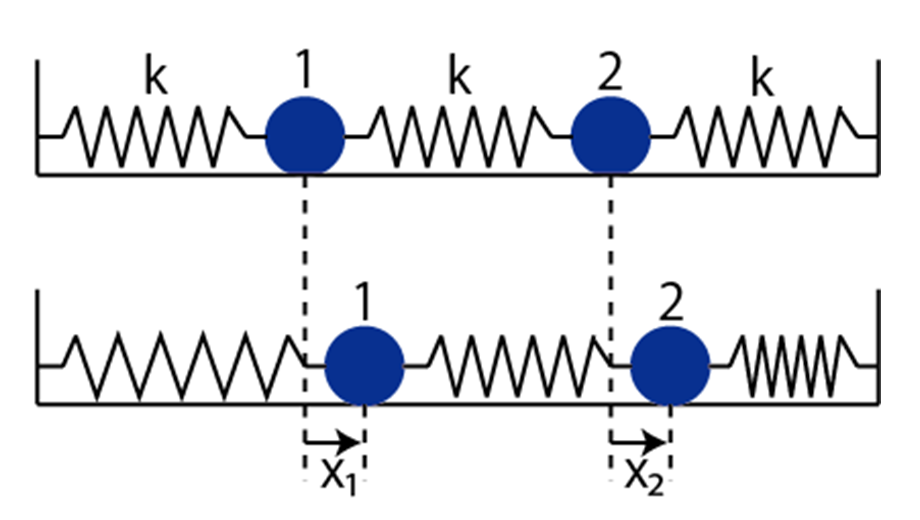
\includegraphics[scale=.20]{bane.png}
\end{center}
\end{figure}
\subsubsection{$おもり1,2それぞれの平衡点からの変位をx_1,x_2としておもりの運動方程式を求めよ.$}
\subsubsection{$x_1,x_2の一般解を求めよ.$}


\newpage
\section*{$+\alpha 問題$}
\subsection{$次の1階連立微分方程式を解け.$}
\subsubsection{}
$\left\{ \begin{array}{l}
x'=-x+2y+\cos t \\
y'=2x-y
\end{array} \right.$

\newpage
\subsubsection{}
$\left\{ \begin{array}{l}
{x'}_1=-x_2+\sin t \\
{x'}_2= x_1+\cos t
\end{array} \right.$

\newpage
\subsection{}
\subsubsection{$以下の連立微分方程式を解け.ただし\Omega ,\eta は定数とする.$}
$\left\{ \begin{array}{l}
\ddot{x}-2\Omega \dot{y}=-\eta x  \\
\ddot{y}+2\Omega \dot{x}=0 
\end{array} \right.$
\\
\\

\newpage
\subsection{}
等質量$m$のおもり1,2がバネにつながれている.各バネのバネ定数は図の通り(順に$k,K,k$)である.このとき、おもり1,2のそれぞれの変位を$x_1,x_2$としてそれぞれのおもりの運動方程式は、
\begin{eqnarray*}
\left\{
\begin{array}{l}
m\ddot{x}_1 = -kx_1 + K(x_2-x_1), \\
m\ddot{x}_2 = -kx_2 - K(x_2-x_1),
\end{array}
\right.
\end{eqnarray*}
となる.
初期条件として、おもり1,2の速度をそれぞれ$\dot{x}_1 = 2\sqrt{(k + K)/m},\ \dot{x}_2 = -2\sqrt{K/m}$としたときの
$x_1(t),~x_2(t)$を求めよ.
\begin{figure}[htpb]
\begin{center}
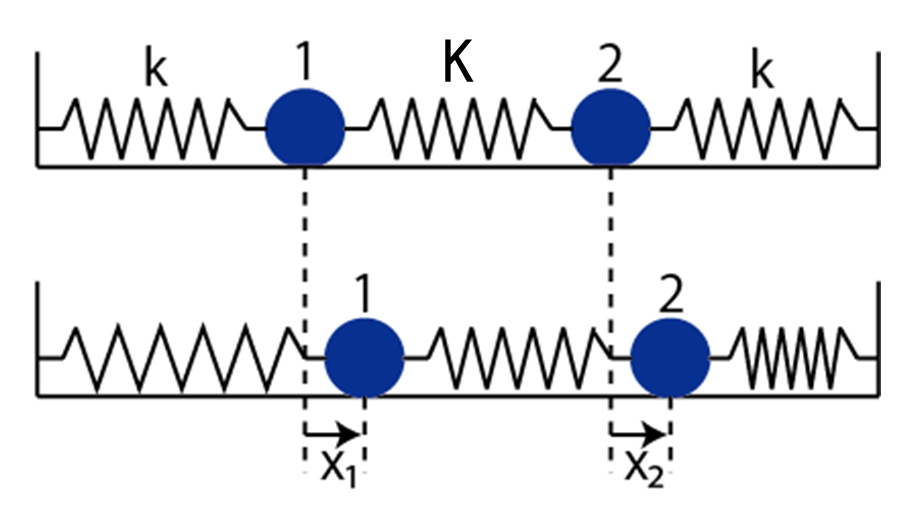
\includegraphics[scale=.20]{bane2.png}
\end{center}
\end{figure}

\newpage
\subsubsection*{$(解答欄つづき)$}

\newpage
\subsection{$動物生態学では、カナダオオヤマネコの個体数と野ウサギの個体数が10年程度の時間で振動することが知られている。以下、このダイナミクスを簡単なモデルで数理化することを考える。$}
被食者(野ウサギ)の個体数を$X$、捕食者(カナダオオヤマネコ)の個体数を$Y$とおく。ここで個体数は実数で近似する。
被食者は草食動物で、自然出生率に応じて$\frac{dX}{dt}=AX$にて指数関数的に増殖する。ただし捕食者があると、その数に比例して食われるために、個体数変化には$-BXY$の減少効果が見込まれる。\par
一方、捕食者$Y$の増加率は被食者数に比例する$\frac{dY}{dt}=CXY$と考えられるが、被食者がいなければ自然減少するので、個体数変化には$-DY$の減少効果が含まれる。これらの効果を総合することによって、以下の非線形連立微分方程式が得られる;\\
\\
$\left\{ \begin{array}{l}
\dot{X}=(A-BY)X \\
\dot{Y}=(CX-D)Y
\end{array} \right.$
\\
\\
この方程式はロトカ=ヴォルテラ方程式と呼ばれ、振動解を持つことが知られている。\\
以下の問いに答えよ。

\subsubsection{$この方程式は非線形(XYの項を含む)なので、解析的に解くことが難しい。そこでここでは簡単のため、\dot{X}=\dot{Y}=0を満たす不動点(X,Y)=(D/C,A/B)からのずれ(x,y)=(X-D/C,Y-A/B)を考えることにする。|x|,|y|が小さいとして\mathcal{O}(xy)の項を無視することにより、以下の線形連立微分方程式を導出せよ。$}
$\left\{ \begin{array}{l}
\dot{x}=-\frac{BD}{C}y \\
\dot{y}=\frac{CA}{B}x
\end{array} \right.$

\newpage
\subsubsection{}
$x,y$に関する(1)の微分方程式を解くことによって、$y$が$x$の振動に$\pi /2$だけ遅れて追従することを示せ。

\end{document}